In many areas around the world, air pollution is the leading environmental health risk affecting both the human population and ecology.
The effects of air pollution range from chronic to less severe health impacts to the general population, air pollution has been labelled carcinogenic by the International Agency for Research on Cancer \citep{IARC:2013}, significant economic impacts due to reduced growth rates of vegetation run into billions of euros per year.
Due to these impacts, many governed areas introduced limit values for the most common and severe air pollutants \citep{AQEU:2015}.

Air pollutants can be emitted directly into the atmosphere (\emph{primary pollutants}) or formed from the chemical reactions of other pollutants (\emph{secondary pollutants}).
Over Europe, particulate matter (PM) and tropospheric ozone (\ce{O3}) are the most problematic with up to $93$ and $98$~\% of Europe's urban population exposed to concentrations above the WHO guidelines \citep{AQEU:2015}.

Tackling the high levels of tropospheric ozone is a complex problem as it is secondary pollutant formed from the reactions of emitted nitrogen oxides (\ce{NO_x}~$\equiv$~NO + \ce{NO2}) and volatile organic compounds (VOCs) in the presence of sunlight.
The photochemical nature of ozone production also lends itself to large impacts from meteorological variables such as temperature and wind speed \citep{Jacob:2009}.
Despite reductions to ozone precursors, the EU target value for human health (the EU does not currently have a  limit value for ozone) was exceeded in $65$~\% of the EU member states and Europe's target value for vegetation was exceeded in $27$~\% of the EU-28 agricultural areas \citep{AQEU:2013}.

Air quality (AQ) modelling is an important tool for predicting future air quality under different emission and meteorological scenarios.
Adequately representing the complexity of ozone production is an ongoing challenge for the modelling community.
Representing the numerous inputs in a correct way that is computationally efficient to reproduce observed trends in tropospheric ozone is a challenge for AQ models.

In this work, we shall determine the effects of different representations of specific model inputs on simulated ozone production.
The research questions addressed in this work, relate specifically to the representation of chemistry, inputs of VOC emissions and temperature on ozone production and are detailed further in Sect.~\ref{s:research_questions}.
After determining the effects on ozone production, Chap.~\ref{c:conclusions} frames these effects in the wider view of improving current state of the art AQ modelling of tropospheric ozone.

\section{Ozone} \label{s:ozone}
%atmospheric O3 with budget, lifetime, stratospheric & tropospheric ozone
Ozone is a constituent gas of the atmosphere found in the stratosphere and troposphere, however its atmospheric effects are very different in these distinct regions.
About 90~\% of the atmospheric ozone is present in the stratosphere with a peak mixing ratio of about $12$~ppm \citep{Seinfeld:2006}.
Stratospheric ozone absorbs the sun's ultraviolet radiation with wavelengths between $280$ and $315$~nm, this is extremely important as excess UV radiation may cause skin cancer, cataracts and a suppressed immune system in humans and can also damage land and aquatic ecosystems \citep{WMO:2010}. 

In contrast, tropospheric ozone, found close to the surface, is both a pollutant and a greenhouse gas. 
Increased levels of tropospheric ozone are harmful to humans, plants and other living systems, as high ozone exposure can lead to pulmonary problems in humans and can decrease both crop yields and forest growth \citep{WMO:2010}. 

Globally, tropospheric ozone is formed mainly via photochemical production from the reactions of emitted VOCs and \ce{NO_x}.
However, the Statospere-Troposphere Exchange (STE), which transports ozone from the stratosphere into the troposphere, may also play a role. 
The STE is driven by the Brewer-Dobson circulation \citep{Brewer:1949, Dobson:1956}, a relatively slow circulation (weeks to months) due to planetary wave disturbances in the troposphere \citep{Haynes:1991}.
The circulation causes air to move downward from the stratosphere into the troposphere at the mid and high latitudes and is balanced by upward exchange at the tropics. 
%The STE also has a seasonal variability where the maximum transport occurs during spring \citep{Appenzeller:1996}, due to the increase in altitude of the tropopause - the boundary level between the troposphere and the stratosphere - which moves stratospheric air into the troposphere. 

A spring-time peak in \ce{O3} concentrations is common in the mid-latitudes of the Northern Hemisphere and the STE was thought to be responsible. 
However, it is only very rarely that \ce{O3} originating via STE can influence tropospheric \ce{O3} levels \citep{Lelieveld:2000}. 
It was later realised that this spring maximum is due to the photochemical reactions occuring in the Northern Hemisphere spring after the buildup of reservoir species over winter \citep{Penkett:1986}.
These reservoir species are oxidised photochemically at a faster rate due to the increase in temperature, moisture and sunlight.

%metereology impacts 
Tropospheric \ce{O3} is not only impacted by emission levels, it is also affected by meteorological variables such as temperature, number of hours of sunshine and wind as these impact transport, dry and wet deposition rates and also chemical reaction rates \citep{Hess:2009}.
Meteorology influences both regional and global \ce{O3} \citep{Hess:2009}, climate patterns such as El Ni\~{n}o are also known to impact \ce{O3} levels in certain areas \citep{Sudo:2001}. 
The effects of meteorology on ozone production shall be presented in more detail in Sect.~\ref{s:meteo_ozone}.

In general, there has been great effort to reduce emissions of ozone precursors from anthropogenic sources.
For example, the emissions of non-methane VOCs (NMVOCs) over Europe have decreased by $20$~\% and emissions of \ce{NO_x} have decreased by almost $30$~\% from 2004 levels.
Despite these reductions in ozone precursors, up to $98$~\% of Europe's urban population are exposed to levels of ozone exceeding the WHO guidelines \citep{AQEU:2015}.

Modelling of \ce{O3} production has played a part in understanding the complexity of atmospheric chemistry, such as the non-linear relationship of \ce{O3} production on the concentrations of VOCs and \ce{NO_x}.
The results of these modelling experiments can be used to produce more effective strategies for reducing ozone levels.
The need for more effective air quality standards in turn also drives the model development and deeper understanding of the atmospheric processes controlling ozone production.
In this work, we shall address the representation of three important parts of an AQ model (chemistry, NMVOC emissions and meteorology) and their impacts on simulated ozone production.

\section{Ozone Production Chemistry} \label{s:ozone_chemistry}
%O3 chemical sources & sinks, linking VOCs.
Troposperic ozone is principally formed by the photolysis of nitrogen dioxide (\ce{NO2}), which produces nitrogen oxide (NO) and a ground state oxygen atom (\ce{O(^3P)}), this then reacts with molecular oxygen (\ce{O2}) to form \ce{O3}. 
Ozone reacts rapidly with NO to return \ce{NO2} and \ce{O2}, this is represented by the following reaction cycle.
\begin{rxnarray}
    \ce{NO2 + h\nu} & \rightarrow \ce{NO + O(^3P)} \label{r:NO2_hv} \\
    \ce{O(^3P) + O2} & \xrightarrow[]{\text{\tiny{M}}} \ce{O3} \label{r:O_O2} \\
    \ce{NO + O3} & \rightarrow \ce{NO2 + O2} \label{r:NO_O3}
\end{rxnarray}

These reactions do not produce net \ce{O3}, due to a photoequilibrium between NO, \ce{NO2} and \ce{O3} \citep{Atkinson:2000}. 
Adding VOCs of both biogenic and anthropogenic origin, such as methane (\ce{CH4}), and other gas-phase compounds, such as carbon monoxide (CO) - to the mix, results in net \ce{O3} production. 
The oxidation mechanism of CO, taking into account reactions that give maximum \ce{O3} yield, is
\begin{rxnarray}
    \ce{CO + OH} & \xrightarrow[]{\ce{O2}} \ce{CO2 + HO2} \label{r:CO_OH} \\
    \ce{HO2 + NO} & \rightarrow \ce{NO2 + OH} \label{r:HO2_NO} 
\end{rxnarray}
whilst the oxidation mechanism of \ce{CH4} with maximum \ce{O3} yield is
\begin{rxnarray}
    \ce{CH4 + OH} & \xrightarrow[]{\ce{O2}} \ce{CH3O2 + H2O} \label{r:CH4_OH} \\
    \ce{CH3O2 + NO} & \xrightarrow[]{\ce{O2}} \ce{HCHO + HO2 + NO2} \label{r:CH3O2_NO} \\
    \ce{HCHO + hv} & \xrightarrow[]{\ce{O2}} \ce{2 HO2 + CO} \label{r:HCHO_hv} 
\end{rxnarray}
taking into account the net result for the CO oxidation mechanism, the net yield for \ce{CH4} is
%\begin{rxnarray}
%    \reactionitem{\ce{CH4 + 10 O2}}{\ce{CO2 + H2O + 2 OH + 5 O3}.}{new}{r:netCH4}
%\end{rxnarray}
Both mechanisms are taken from \citep{Seinfeld:2006}.

To summarise, oxidation of VOCs results in the formation of peroxy radicals which then convert NO to \ce{NO2} and both \eqref{r:NO2_hv} and \eqref{r:O_O2} proceed. 
These oxidation mechanisms are linked in the sense that the \ce{CH4} mechanism gives a maximum \ce{O3} yield, once the mechanism of CO is also included. 

Since these mechanisms produce the maximum \ce{O3} yield, the reactions that cause \ce{O3} destruction or inhibit its production are not included. 
It should also be noted that some reactions can follow more than one pathway that is indicated above and that products from these pathways can be removed from the atmosphere via deposition processes. 
Thus, the maximum \ce{O3} yield outlined in reactions %\eqref{r:netCO} and \eqref{r:netCH4} is not reached in the atmosphere.

Another aspect of \ce{O3} production is its dependence on the atmospheric concentrations of both VOCs and nitrogen oxides (\ce{NO_x = NO + NO2}) and this also influences the reaction pathways. 
Moreover, the precursors of ozone are linked to anthropogenic activity, hence a so-called weekend effect (i.e. there is a reduction on \ce{O3} concentration over the weekend) is also evident (see for example, \citep{Koo:2012}). 
Further discussion on the balance of VOC and \ce{NO_x} concentration to \ce{O3} production shall be given in Section \ref{s:VOC&NOx}.

\subsection{Chemical Families}

A concept that is extremely useful in atmospheric chemistry is that of a chemical family. 
This is used to describe two or more compounds that form a rapid cycle of production and destruction. 
An example is the cycling between NO and \ce{NO2} in \eqref{r:NO2_hv} and \eqref{r:NO_O3}, hence NO and \ce{NO2} form the nitrogen oxides chemical family \ce{NO_x}.

A chemical family also has its own chemical lifetime, where the chemical lifetime is the average time that a chemical species takes to be removed - by reaction or deposition processes - from the atmosphere. 
An equilibrium is reached for the compounds of the chemical family, called a pseudo-steady state, which is then re-balanced when a compound from the family reacts with a species not present in the chemical family.

Examples of important chemical families are given below in Table \ref{t:chemfam} and taken from \citep{Seinfeld:2006}.
\begin{table}
    \begin{center}
        \begin{tabular}{lll}
            \hline \hline
            \textbf{Symbol} & \textbf{Family Name} & \textbf{Components} \\
            \hline \hline
            \ce{NO_x} & Nitrogen oxides & NO + \ce{NO2} \\
            \ce{O_x} & Odd oxygen & \ce{O3 + O + O(^1D) + NO2 + NO3 + N2O5} \\
            \multirow{2}{*}{\ce{NO_y}} & \multirow{2}{*}{Oxidised nitrogen} & \ce{NO + NO2 + HNO3 + N2O5 + ClONO2} \\
            & & \hspace{0.5cm} \ce{ + NO3 + HOONO2 + BrONO2} \\
            \ce{HO_x} & Hydrogen radicals & \ce{OH + HO2} \\
            PAN & Peroxyacyl nitrates & Compounds of general formula \\ 
            & & \hspace{0.5cm} \ce{RC(O)OONO2} \\
            \hline \hline
        \end{tabular}
	\caption{Chemical Families commonly used in Tropospheric Chemistry \citep{Seinfeld:2006}}
	\label{t:chemfam}
    \end{center}
\end{table}

\subsection{Reservoir Molecules} \label{s:reservoir}

Compounds that react with radicals or \ce{NO_x} are called reservoir molecules. 
These will slow down \ce{O3} production and if they have a sufficiently long enough lifetime, can also transport and then release radicals or \ce{NO_x} to promote \ce{O3} formation in a separate location. 
For example, hydrogen peroxide (\ce{H2O2}) is a reservoir molecule for \ce{HO_x} as shown in the below sequence of reactions \citep{Seinfeld:2006}.
\begin{rxnarray}
    \ce{HO2 + HO2} & \rightarrow \ce{H2O2 + O2} \label{r:HO2_HO2} \\
    \ce{H2O2 + h\nu} & \rightarrow \ce{OH + OH} \label{r:H2O2_hv} \\
    \ce{H2O2 + OH} & \rightarrow \ce{H2O + HO2} \label{r:H2O2_OH}
\end{rxnarray}

Nitrous acid (HONO) is a reservoir molecule for \ce{NO_x} and \ce{HO_x}, formed by a heterogeneous reaction of \ce{NO2} and \ce{H2O}. 
HONO can be formed during night-time and then photodissociates at sunrise to regenerate OH and NO \citep{Seinfeld:2006}.
\begin{rxnarray}
    \ce{HONO + h\nu} & \rightarrow \ce{OH + NO} \label{r:HONO_hv}
\end{rxnarray}

An important class of reservoir molecules are ther peroxyacyl nitrates (PANs) of general formula \ce{RC(O)OONO2}. 
The first compound in this class, \ce{CH3C(O)OONO2}, is also called PAN and can be formed by reactions of peroxyacetyl radicals with \ce{NO2}, PAN then thermally dissociates to return the reactants \citep{Kleinman:2005}.
\begin{rxnarray}
    \ce{CH3C(O)O2 + NO2} & \xrightarrow[]{\text{M}} \ce{CH3C(O)O2NO2} \label{r:CH3CO3_NO2}
\end{rxnarray}
PAN's lifetime is dependent on meteorology due to a strong temperature dependence \citep{Moxim:1996}. 
This can lead to situations where \ce{NO_x} is transported to different regions and then released by dissociation. 
PAN is thought to have a regional rather than a global influence on the \ce{NO_x} budget \citep{Moxim:1996}.

\subsection{Volatile Organic Compounds}
%VOCs to be considered
Table lists Non-Methane Volatile Organic Compounds (NMVOCs) that are emitted from US cities \citep{Baker:2008}. 
The mean is calculated from \citep{Baker:2008} using the total of 31 data points from 28 cities in the United States. 
Of these NMVOCs there is only one which has a primarily biogenic source and this is isoprene (2-methyl 1,3-butadiene). 
Although not evident from Table, biogenic VOCs are globally the most abundant VOCs \citep{Goldstein:2007}. 
Since the data in Table are mainly taken from urban cities, the impact of anthropogenic emissions outweigh those of the biogenic sources \citep{Baker:2008} - although isoprene has some anthropogenic sources (see \citep{Borbon:2003}). 

The sources of the alkanes listed below are natural gases, liquified petroleum gas (LPG), combustion and industry, for the case of octane, vehicle exhaust is also a source. 
Alkene sources are mainly due to industrial activities and vehicular emissions. 
Aromatic compounds are mainly due to vehicle emissions, while benzene and toluene are also emitted due to industrial activity and combustion is also a further source for benzene \citep{Arsene:2009}.

%reactivity of species - Atkinson
Alkanes are saturated hydrocarbons, meaning that all bonds between carbon and hydrogen atoms are single bonds, resulting in slow reacting species. 
The dominant tropospheric process for alkanes is reaction with the hydroxyl (OH) radical, but they also react with the nitrate (\ce{NO3}) radical and chlorine atoms. 
The presence of a double bond in alkenes and a triple bond in alkynes leads to increased reactivity. 
In the troposphere both alkenes and alkynes react with the OH radical, the \ce{NO3} radical and also with \ce{O3}. 
Aromatic compounds react with the OH and \ce{NO3} radicals. 
Hence it can be noted that the key reactive species in the troposphere is the OH radical as it reacts with practically all organic compounds, the exceptions being chlorofluorocarbons (CFCs) and halons without hydrogen atoms. 

Reaction with the OH radical is predominant during the day, since it is formed mainly by photolysis, during the night there is an increase in the \ce{NO3} radical concentration and so reaction rates with this radical are increased. 
The reason for this increased night-time concentration of the \ce{NO3} radical is that during the day the reaction that forms \ce{NO3} 
\begin{rxnarray}
    \ce{NO2 + O3} \rightarrow \ce{NO3 + O2}
\end{rxnarray}
is balanced by the quick photolysis of \ce{NO3}
\begin{rxnarray}
    \ce{NO2 + h\nu} & \rightarrow \ce{NO + O2} \label{r:NO3_hva} \\
    \ce{NO2 + h\nu} & \rightarrow \ce{NO2 + O(^3P)} \label{r:NO3_hvb} 
\end{rxnarray}
The main photolysis pathway is via reaction \eqref{r:NO3_hvb} which occurs about 90~\% of the time.
However, during night-time photolysis does not occur and hence there is a buildup of \ce{NO3} radicals \citep{Atkinson:1990, Atkinson:2000}.

\subsection{VOC Chemistry}
%atmospheric chemistry of NMVOCs 
Figure \ref{f:VOC_reaction} represents a general and simplified reaction scheme for VOCs in the troposphere. 
Although there are many different VOC classes involved in tropospheric chemistry, there are many similarities between their reaction schemes. 
This shall be summarised below however for more a more detailed description of tropospheric chemistry, \citep{Atkinson:2000} should be consulted. 
\begin{figure}
    \begin{center}
        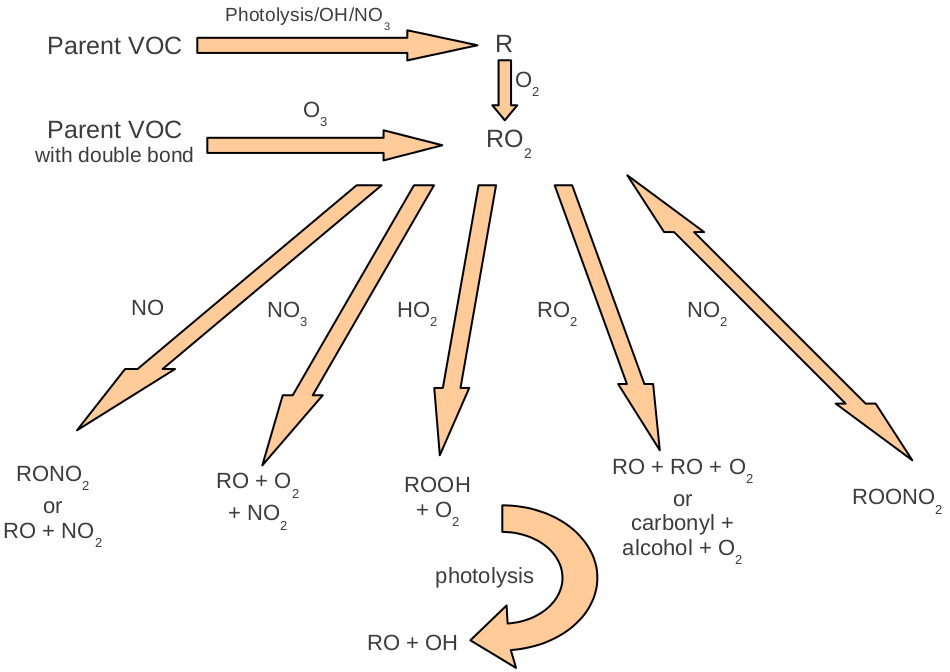
\includegraphics[height=100mm, width=120mm]{VOC_reaction_updated}
        \caption[what is this]{VOC reaction pathway}
        \label{f:VOC_reaction}
    \end{center}
\end{figure}

As noted earlier, the most common initiation reaction of a VOC is with the OH radical, and this forms an alkyl or substituted alkyl radical (R) depending on the parent VOC. 
The addition reaction with \ce{O2} then leads to the formation of alkyl peroxy radicals (\ce{RO2}). 
During the night-time, reaction with the \ce{NO3} radical is of importance and for VOCs containing a double bond, reaction with \ce{O3} also occurs. 
Photolysis is an important degradation initiator for carbonyl species, this is particularly important throughout the whole degradation mechanism of the VOC as carbonyl species, such as formaldehyde, are common reaction products. 
These initial reaction pathways all lead to the formation of \ce{RO2} radicals, as shown below.
\begin{rxnarray}
    \ce{VOC + OH / NO3 / O3 / h\nu} & \rightarrow \ce{R} \label{r:VOC_init} \\
    \ce{R + O2} & \rightarrow \ce{RO2} \label{r:R_O2}
\end{rxnarray} 
\ce{RO2} radicals can subsequently react with NO, \ce{NO2}, hydroperoxy (\ce{HO2}) radicals, \ce{NO3} radicals - mainly during night-time - and also with other alkyl peroxy radicals. 
The competition between these reactions determines the amount of net ozone production or loss from the parent VOC. 
\begin{rxnarray}
    \ce{RO2 + NO} & \xrightarrow[]{\text{M}} \ce{RONO2} \label{r:RO2_NOa} \\
    \ce{RO2 + NO} & \rightarrow \ce{RO + NO2} \label{r:RO2_NOb} \\
    \ce{RO2 + NO2} & \xrightarrow[]{\text{M}} \ce{ROONO2} \label{r:RO2_NO2} \\
    \ce{RO2 + HO2} & \rightarrow \ce{ROOH + O2} \label{r:RO2_HO2} \\
    \ce{RO2 + NO3} & \rightarrow \ce{RO + NO2 + O2} \label{r:RO2_NO3} \\
    \ce{RCH(OO)R` + RCH(OO)R`} & \rightarrow \ce{RCH(O)R` + RCH(O)R` + O2} \label{r:RCHOOR_RCHOORa} \\
    \ce{RCH(OO)R` + RCH(OO)R`} & \rightarrow \ce{RCH(OH)R` + RC(O)R` + O2} \label{r:RCHOOR_RCHOORb}
\end{rxnarray}
All pathways in Figure \ref{f:VOC_reaction} that lead to \ce{NO2} formation can result in \ce{O3} formation due to \eqref{r:NO2_hv} and \eqref{r:O_O2}. 
Reaction with the \ce{HO2} radical results in the formation of hydroperoxides (ROOH), which then photolyse to an alkoxy (RO) radical and the OH radical, this OH radical is then available to react with other VOCs. 
The carbonyl and alcohol products resulting from reaction with other \ce{RO2} radicals will follow a similar sequence of reactions and hence can also produce further \ce{O3}. 
Reaction with \ce{NO2} leads to the formation of alkyl peroxynitrates (\ce{ROONO2}), however this reaction product can be thermally unstable and may decompose quickly to the reactants, as mentioned in Section \ref{s:reservoir}.

The RO radical that results from many of the \ce{RO2} pathways undergoes further reactions, either by decomposition, isomerisation or reaction with \ce{O2}. 
The products that result from the reaction pathways depend on the parent VOC and this also determines the number of NO-to-\ce{NO2} conversions, eventually leading to \ce{O3} formation.

All VOCs and their degradation products will ultimately result in carbon dioxide (\ce{CO2}) and water vapour. 
The path that each VOC takes to reach its final products is dependent on the type of VOC, the radical concentration, the \ce{NO_x} concentration and other factors such as time of day and year. 
The detailed atmospheric chemistry of some simple VOCs is well-understood (for example, methane) however for more complex molecules, especially aromatic VOCs, there are a great number of uncertainties. 
These uncertainties can be related to kinetic data, photolysis rates, reaction branching ratios and in most cases the reaction products. 
Any uncertainties in reaction pathways and products of VOCs also leads to uncertainties in the ozone forming potential of the respective VOC \citep{Atkinson:2000}.

\subsection{\texorpdfstring{VOC and \ce{NO_x} Chemistry}{VOC and NOx Chemistry}} \label{s:VOC&NOx}
%balance of NOx & NMVOC for O3 production
As mentioned above, \ce{O3} chemistry is influenced by both VOC and \ce{NO_x} concentrations. 
Figure \ref{f:O3_isopleth} depicts the non-linear relationship between \ce{O3} concentration when considered as a function of VOC concentration (in ppmC, i.e. parts per million mass of a carbon unit of the VOC, \ce{CH_{2.5}}) and \ce{NO_x} concentration (in ppm, i.e. parts per million mass). 
\begin{figure}
	\begin{center}
		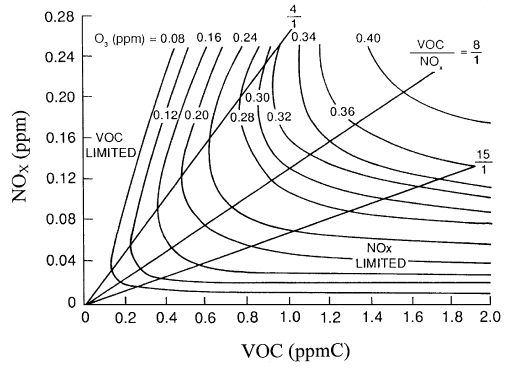
\includegraphics[height=90mm, width=85mm]{O3_isopleth_1.png}
		\caption{Ozone isopleth plots for various initial concentrations of \ce{NO_x} and a specified VOC mixture. Taken from \citep{Jenkin:2000}.}
		\label{f:O3_isopleth}
	\end{center}
\end{figure}

This relationship can be divided into distinct regimes: \textbf{\ce{NO_x}-sensitive}, \textbf{VOC-sensitive} and \textbf{VOC-and-\ce{NO_x}-sensitive}. 
The \ce{NO_x}-sensitive regime is the right-most part, the VOC-and-\ce{NO_x}-sensitive regime is the middle section and the VOC-sensitive regime is the left-most part of Figure \ref{f:O3_isopleth} and these correspond to high, middle and low VOC:\ce{NO_x} ratios, respectively. 
These different regimes arise from how the atmosphere removes \ce{NO_x} and radicals resulting from VOCs. 

In the \ce{NO_x}-sensitive regime, the concentration of \ce{NO_x} is low compared to that of radicals. 
Hence, peroxy radicals are removed by reaction with the OH radical such as 
\begin{rxnarray}
    \ce{HO2 + OH} \rightarrow \ce{H2O + O2} \label{r:HO2_OH}
\end{rxnarray}
or by peroxy radical addition reactions.

This results in the NO concentration controlling the number of NO-to-\ce{NO2} conversions, rather than the concentration of peroxy radicals produced during VOC oxidation. 
An increase in NO conversion would thus promote \ce{O3} production due to an increase in \eqref{r:NO2_hv} and \eqref{r:O_O2} reactions. 
Increasing VOC concentrations would not increase \ce{O3} production as this only speeds up the formation of peroxy radicals and has no direct effect on the \ce{NO_x} concentration.

The VOC-sensitive regime corresponds to high \ce{NO_x} concentrations, hence radicals will tend to react with either NO or \ce{NO2}. 
Increasing \ce{NO_x} concentrations will not increase not increase \ce{O3} production as the \ce{NO_x} will react with the peroxy radicals resulting from VOC degradation. 
However, this increase in \ce{NO_x} increases the formation of nitric acid (\ce{HNO3}) by reaction with the OH radical \citep{Kleinman:1991, Kleinman:1994, Kirchner:2001}.
\begin{rxnarray}
    \ce{NO2 + OH} \rightarrow \ce{HNO3} \label{r:NO2_OH}
\end{rxnarray}
The competition of VOCs and \ce{NO_x} for reaction with the OH radical is at the heart of \ce{O3} production or destruction in the VOC-sensitive regime. 
Reaction of VOCs with the OH radical will produce more peroxy radicals, increasing \ce{O3} production whilst reaction of \ce{NO_x} increases \ce{HNO3} by \eqref{r:NO2_OH} which reduces \ce{O3} production \citep{Kleinman:1991, Kleinman:1994, Kirchner:2001}.

The VOC-and-\ce{NO_x}-sensitive regime is characterised by \ce{O3} production being sensitive to both VOC and \ce{NO_x} concentrations. 
The turning point from a VOC-sensitive to a VOC-and-\ce{NO_x}-sensitive regime is when the maximum \ce{O3} production for a particular VOC concentration has been reached. 
The shift into a \ce{NO_x}-sensitive occurs when increases in VOC concentrations result in very little \ce{O3} production \citep{Kirchner:2001}. 
The non-linear relationship can be thought of as a titration process between the amount of radicals and the \ce{NO_x} present in the atmosphere.

This non-linear nature of the atmosphere must be taken into account when policymakers consider control strategies for \ce{O3} concentrations. 
The difficulty is exacerbated by the fact that regions can alternate between these regimes depending on the season, time of day etc. 

Moreover, an air parcel emitted in an urban area may also evolve as outlined in Figure \ref{f:air_parcel}, as it moves downwind. 
\begin{figure}
	\begin{center}
		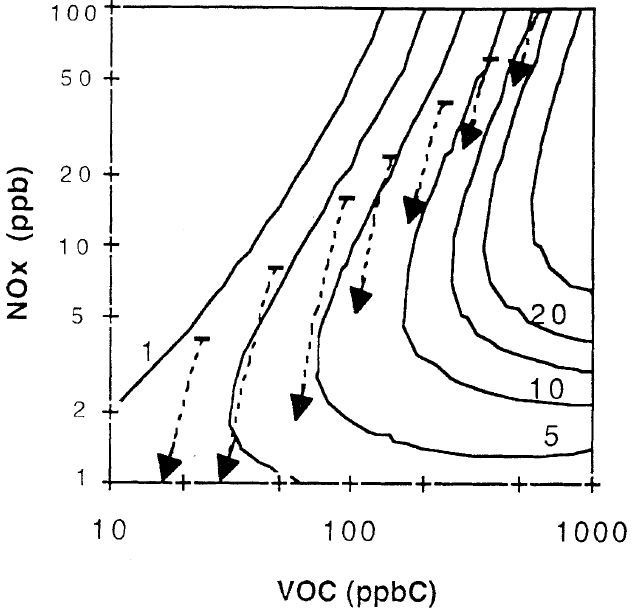
\includegraphics[height=80mm, width=75mm]{air_parcel.png}
		\caption{Air parcel evolution overlayed with ozone isopleth plots for various initial concentrations of \ce{NO_x} and VOCs. Taken from \citep{Sillman:1999}.}
		\label{f:air_parcel}
	\end{center}
\end{figure}
Once the air parcel has been emitted, it would typically fall into the VOC-sensitive regime but as the parcel ages it would move into the \ce{NO_x}-sensitive regime. 
Reducing VOC and \ce{NO_x} would reduce tropospheric \ce{O3}, whilst reducing VOC levels would only be effective during VOC-sensitive regimes and reducing \ce{NO_x} levels is only effective in \ce{NO_x}-sensitive regimes and can even increase \ce{O3} concentrations \citep{Sillman:1999}. 
This is due to the radical or \ce{NO_x} removal pathways that may or may not promote \ce{O3} production as discussed above.

\section{Emissions of Ozone Precursors} \label{s:precursor_emissions}

\section{Effects of Meteorology on Ozone Production} \label{s:meteo_ozone}

The effect of meteorology is an aspect of atmospheric chemical transport modelling that needs to be taken into account. 
However it is also frequently the major source of uncertainty for the calculated \ce{O3} concentrations. 
Wind speeds in particular may lead to under- or over-predicated values of \ce{O3} concentrations \citep{Sillman:1999}. 

\section{Research Questions} \label{s:research_questions}

